\ylDisplay{Maja} % Ülesande nimi
{Autor} % Autor
{lõppvoor} % Voor
{2013} % Aasta
{P 6} % Ülesande nr.
{3} % Raskustase
{
% Teema: Soojusõpetus

\ifStatement
Maja koosneb kahest ühesugusest toast, mis on sümmeetrilised neid eraldava vaheseina suhtes. Mõlemas toas on radiaator võimsusega $P$. Väljas on temperatuur $T_0$. Kui lülitada sisse üks radiaator, siis pärast soojenemist on temperatuur radiaatoriga toas $T_1$ ja teises $T_2$. Leidke temperatuur $T_3$, milleni soojenevad toad, kui töötavad mõlemad radiaatorid. Eeldage, et soojusvahetuse võimsus pinnaühiku kohta on võrdeline temperatuuride vahega. Põrand ja lagi on hästi soojustatud. 
\begin{center}
	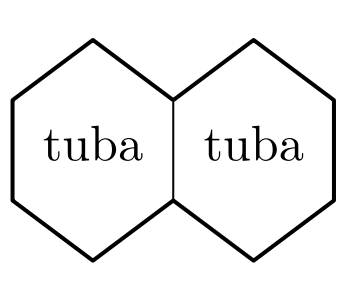
\includegraphics[width=0.5\linewidth]{2013-v3p-06-yl.PNG}
\end{center}
\fi

\ifHint
Ülesannet on võimalik lahendada, kui avaldada tundmatu võrdetegur kuna soojusvahetuse võimsus pinnaühiku kohta on võrdeline temperaturride vahega peab ka soojusvahetus läbi terve seina olema võrdeline temperatuuride vahega. Ülesannet on ka võimalik lahendada lihtsamini kui märkame, et tegu on lineaarse süsteemiga ja teame, et lineaarse süsteemi korral kahe lahendi superpositsioon on samuti süsteemi lahend.
\fi

\ifSolution
Võtame, et soojusvahetuse võimsus läbi toa välisseina on
\begin{center}
$W_v = x(T_{tuba} - T_0)$,
\end{center}
kus $x$ on tundmatu võrdetegur - kuna soojusvahetuse võimsus pinnaühiku kohta on võrdeline temperaturride vahega peab ka soojusvahetus läbi terve seina olema võrdeline temperatuuride vahega. Samamoodi võtame, et soojusvahetuse võimsus läbi siseseina on
\begin{center}
$W_s = y(T_{1. tuba} - T_{2. tuba})$.
\end{center}
Kui töötab ainult üks radiaator, saame kirjutada mõlema toa jaoks võrrandi tingimusest, et soojushulk tubades ei muutu.
\begin{center}
$P = x(T_1 - T_2) + y(T_1 - T_2)$
\end{center}
\begin{center}
$y(T_1 - T_2) = x(T_2 - T_0)$.
\end{center}
Lahedndades saame, et $x = \frac{P}{T_1 + T_2 + 2T_0}$. Kui töötavad mõlemad radiaatorid, siis summarset soojusvahetust läbi vaheseina pole. Mõlema toa jaoks kehtib siis võrrand $P = x(T_3 - T_0)$. Siit avaldame
\begin{center}
$T_3 = (T_1 + T_2 - T_0)$.
\end{center}

Lihtsam lahendus:
Ülesannet on ka võimalik lahendada lihtsamini kui märkame, et tegu on lineaarse süsteemiga ja teame, et lineaarse süsteemi korral kahe lahendi superpositsioon on samuti süsteemi lahend. Käesoleval juhul on üheks lahendiks, et kui ühes toas töötab radiaator $P$, siis soojenevad toad $\triangle T_1 = T_1 - T_0$ ja $\triangle T_2 = T_2 - T_0$ võrra. Võttes teiseks lahendiks esimese lahendi peegelpildi, saame superpositsioonina, et kui töötavad mõlemad radiaatorid, soojenevad mõlemad toad $\triangle T_3 = T_2 - T_0 + T_1 - T_0$ võrra, ehk $T_3 = (T_1 + T_2 - T_0)$. 
\fi
}